\documentclass[10pt]{article}
\usepackage[margin=2.2cm]{geometry}
\usepackage{amsmath,amssymb}
\usepackage{graphicx}
\usepackage{booktabs}
\usepackage{multirow}
\usepackage[dvipsnames]{xcolor}
\usepackage[colorlinks=true,linkcolor=NavyBlue,citecolor=NavyBlue]{hyperref}
\usepackage{enumitem}
\setlength{\parskip}{0.35em}
\setlength{\parindent}{0pt}

\newcommand{\Fpro}{F_\mathrm{pro}}
\newcommand{\TG}{T_G}

\title{\vspace{-1.5em}Noise-tailored two-qubit gates on an experimentally
anchored dephasing model\vspace{-0.4em}}
\author{Qasim Khan}
\date{June 11, 2026}

\begin{document}
\maketitle
\vspace{-1.8em}

\textit{This note retells the paper's pipeline on the new experimentally
anchored noise model: where the spectra come from and why, what the
frequency-comb QNS protocol recovers, what the gate optimizer actually uses
of that knowledge, and what the noise-tailored gates deliver. Throughout,
the optimizer never sees ground truth, and every quoted ``true'' infidelity
is evaluated exactly on the analytic model. All numbers regenerated June 11,
2026.}

\section{The noise model: what we assume, and why}\label{sec:model}

The synthetic spectra of the earlier drafts have been replaced by a model in
which every structural feature is imported from a published measurement on
semiconductor spin qubits. The skeleton is the Tarucha-group Si/SiGe pair
[Yoneda \emph{et al.}, Nat.\ Phys.\ \textbf{19}, 1793 (2023)], to date the
only experiment that has measured \emph{all six} auto- and cross-spectra of
the two qubit splittings and the exchange coupling, which is exactly the
object our QNS protocol reconstructs.

\textbf{Two correlated local fields, not one shared bath.} Yoneda's central
structural finding fixes the form of the model. The measured inter-qubit
coherence is large but partial ($|c_{12}|$ up to $0.7$), the
qubit-1--exchange coherence is in-phase, and the qubit-2--exchange coherence
is \emph{anti}-phase. That $(+,+,-)$ sign pattern is impossible for a single
shared noise source, which forces all three signs positive. The minimal
structure that reproduces it, validated in the same experiment, is two
partially correlated \emph{local} electric fields $e_A, e_B$ (shared
fraction 0.8 here), with the exchange coupling responding to their
\emph{difference}, plus an independent nuclear process on each qubit:
\begin{equation*}
\zeta_1 = e_A + n_1, \qquad
\zeta_2 = e_B + n_2, \qquad
\zeta_{12} = a\, e_A - b\, e_B, \quad b \gtrsim a .
\end{equation*}
This is physical ($J$ responds to the interdot potential tilt) and it pins
the signs and relative phases of all three cross-spectra rather than leaving
them free. The achieved in-band coherences are $|c_{12}| = 0.67$,
$c_{1,12} = 0.28+0.50i$, and $c_{2,12} = -0.43+0.44i$, reproducing the
measured pattern. Because no cross-spectral data exists above $\sim$Hz, the
imaginary parts are generated by a small causal lag on the shared component
of $e_B$; this is a stated modeling choice, and it usefully forces the
reconstruction to recover $\mathrm{Im}\,S$ at the 10--30\% level rather than
being handed real spectra.

\textbf{Spectral shapes.} The in-band charge-noise exponents are taken from
natural-Si spectroscopy [Rojas-Arias \emph{et al.}, npj QI (2025)]:
$S_{el} \sim \omega^{-0.7}$ on qubit 1 and $\omega^{-0.4}$ on qubit 2. The
qubit asymmetry is itself a measured feature, and exponents in this range
are corroborated across platforms (GaAs exchange noise shows
$\omega^{-0.7}$ [Dial \emph{et al.}, PRL \textbf{110}, 146804 (2013)]). The
local nuclear component is steeper ($\sim\omega^{-1.2}$) and weighted heavier
on qubit 2, mirroring Yoneda's qubit B, which carried excess uncorrelated
nuclear noise; it is what makes the coherences come out partial rather than
perfect.

\textbf{Amplitude anchor.} Rather than unit-converting published
$\mathrm{kHz^2/Hz}$ values across one-sided/two-sided and angular-frequency
conventions, the absolute scale is set by a coherence target: $T_2^{*} =
800\,\tau = 20\,\mu$s per qubit at the $\tau = 25$\,ns anchor, the
purified-$^{28}$Si value [Yoneda \emph{et al.}, Nat.\ Nanotech.\ \textbf{13},
102 (2018)]. The model then \emph{outputs} a Gaussian FID $T_2 \approx
771\,\tau \approx 19\,\mu$s. The gate windows studied sit at
$0.05$--$3.3\,T_2$ for the entangling gate and reach $13\,T_2$ for the
longest idles; they bracket the regime where dephasing goes from
perturbative to dominant.

\textbf{The $ZZ$ channel: the most consequential choice.} Yoneda measured
exchange noise at the symmetric point, where it is a factor $\sim 3\times
10^{-4}$ below the qubit noise; a model calibrated there would render the
two-qubit channel irrelevant by construction. A two-qubit \emph{gate},
however, operates away from that sweet spot. We therefore calibrate
$S_{12,12}$ at the gate operating point using Dial's GaAs exchange-noise
measurements: relative $J$-noise is scale-invariant ($dJ/d\varepsilon \propto
J$) with echo quality factors $Q \sim 600$, which puts coupler noise one to
two orders below qubit noise \emph{at operating} $J$. We set the in-band
ratio $S_{12,12}/\sqrt{S_{1,1}S_{2,2}} = 0.10$ (exponent $0.7$, Dial). This
is the model's single most important free knob: it decides how much of the
error budget the two-qubit channels can claim, and $0.05$--$0.15$ is the
defensible range around our choice.

\textbf{The featured regime: nuclear-difference lines.} On top of this
monotonic (``bland'') background, the featured regime adds the one sharp
spectral structure measured in this class of devices: the triplet of narrow
lines at \emph{differences} of nuclear Larmor frequencies, observed in GaAs
[Malinowski \emph{et al.}, Nat.\ Nanotech.\ \textbf{12}, 16 (2017)] as two
nearly degenerate lines plus one at twice their frequency, with positions
proportional to $B$. Placed at an effective $B = 600$\,mT they land at
$1.66/1.74/3.40$\,MHz ($\omega\tau = 0.261/0.273/0.534$), inside our
sampling band; widths are set at the comb's resolution limit (physical lines
are narrower). The physics that matters downstream: nuclear noise is
\emph{qubit-local}, and $J$-noise is electrical (Yoneda's central
conclusion), so the lines live on $S_{1,1}$ and $S_{2,2}$ but \emph{not} on
$S_{12,12}$, and the inter-qubit coherence \emph{dips} at the line
frequencies. The cross-spectra are not a scaled copy of the self-spectra;
whether that structure must be measured, and what it costs to ignore it, is
quantified in Sec.\,\ref{sec:design}. (We transpose the measured spectral
\emph{shape class}, a power-law background plus narrow MHz lines of the kind
DD passbands collide with, into our linear-dephasing model; we do not claim
to model the $S$-$T_0$ microscopics behind it.)

One caveat, visible as the shaded region in Fig.~\ref{fig:model}: the
published PSD measurements reach $\sim$1\,MHz, the lower half of our
0.25--5\,MHz sampling band; above that, the power laws are extrapolated. An
infrared cutoff at $\omega\tau = 0.02$ keeps $S(0)$ finite, which is what the
DC slope-fit protocol measures.

\begin{table}[h!]
\centering\small
\begin{tabular}{lll}
\toprule
quantity & value & anchor \\
\midrule
time unit (min.\ pulse separation) & $\tau = 25$ ns & legacy anchor \\
$T_2^{*}$ (both qubits) & $800\,\tau = 20\,\mu$s & purified $^{28}$Si \\
Gaussian FID $T_2 = 2/S_{a,a}(0)$ & $771\,\tau$ / $770\,\tau \approx 19.3\,\mu$s & model output \\
charge-noise exponents & $\omega^{-0.7}$ (Q1) / $\omega^{-0.4}$ (Q2) & natural-Si spectroscopy \\
electrical fraction at $\omega\tau=0.35$ & 0.88 (Q1) / 0.80 (Q2) & Yoneda 2023 structure \\
nuclear-difference lines & $\omega\tau \in \{0.261, 0.273, 0.534\}$ & Malinowski fingerprint \\
 & $= 1.66 / 1.74 / 3.40$ MHz & (two near-degenerate $+$ one at $2\times$) \\
$ZZ$-channel coupling & $S_{12,12}/\sqrt{S_{1,1}S_{2,2}} = 0.1$, $\gamma_J = 0.7$ & Dial operating-point $J$-noise \\
gate windows studied & CZ: $\TG = 40$--$2560\,\tau$; idle: $320$--$10240\,\tau$ & $0.05$--$13\,T_2$ \\
\bottomrule
\end{tabular}
\caption{The dephasing scale and where the gates sit relative to it.}
\label{tab:anchor}
\end{table}

\begin{figure}[h!]
\centering
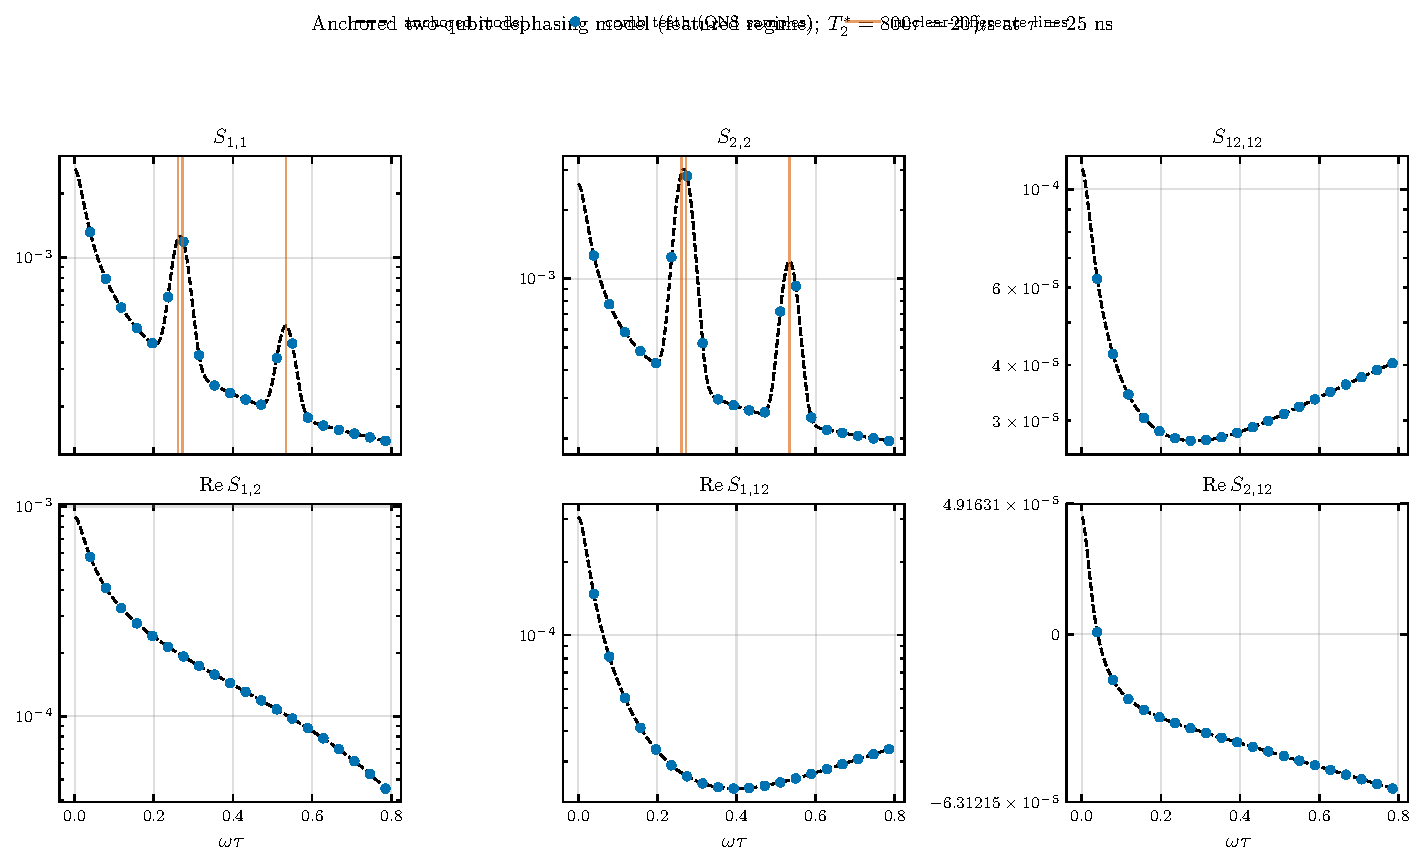
\includegraphics[width=\linewidth]{figs/fig_model_spectra.pdf}
\caption{The anchored two-qubit dephasing model (featured regime). Each panel
is one of the six spectra the QNS protocol reconstructs: the dashed black
curve is the analytic model (top row: the two single-qubit channels and the
$ZZ$ channel; bottom row: the three cross-spectra, with real parts in
black/blue and imaginary parts in green). Blue dots mark the 20 harmonics
$\omega_k\tau = 2\pi k/160$ of the frequency comb, the points the protocol
actually samples, and the open diamond at $\omega = 0$ is the DC point,
measured by dedicated slope-fit (self-spectra) and double-echo ($S_{12,12}$)
experiments. Vertical orange lines: the nuclear Larmor-difference triplet,
which appears on the qubit-local channels only; $J$-noise is electrical,
so $S_{12,12}$ is smooth and the inter-qubit coherence dips at the line
frequencies. Grey shading: frequencies above the published measurement
window, where the model's power-law exponents are extrapolated.}
\label{fig:model}
\end{figure}

\section{Characterization: the blind reconstruction recovers the truth}\label{sec:char}

The model above is what the simulated experiments draw their noise from; the
question is what the comb protocol gets back. The full blind pipeline
(harmonic comb inversion, line/tail/head-aware unfolding, DC points from
noise-aware slope fits and the double-echo $S_{12,12}(0)$ experiment) was
run at 64{,}000 shots per sequence, three ways on identical noise: a
SPAM-free reference, an unmitigated (raw) arm, and a SPAM-mitigated arm.
Everything downstream in this note (gate curves, margin bands, design
experiments) is built on these 64k reconstructions, so all numbers sit on
an equal footing.

The reference reconstruction is accurate at the percent level on the
single-qubit spectra and at 3--6\% on the weaker two-qubit channels
(Table~\ref{tab:recon}), with one caveat the table makes visible: on
$S_{12,12}$ the median pull reaches $1.2$ and the $2\sigma$ coverage drops
to $76\%$. At 64k shots the statistical bars have shrunk to the point where
the unfolding systematic on the weakest channel is no longer fully covered
by the quoted uncertainty. The other five channels remain covered
($\geq 95\%$ within $2\sigma$, median pulls $\leq 0.6$).

\begin{table}[h!]
\centering\small
\begin{tabular}{lcccc}
\toprule
spectrum & median rel.\ dev. & median pull & max pull & within $2\sigma$ \\
\midrule
$S_{1,1}$    & 1.3\% & 0.37 & 2.7 & 95\% \\
$S_{2,2}$    & 1.1\% & 0.31 & 1.6 & 100\% \\
$S_{12,12}$  & 6.3\% & 1.24 & 3.1 & 76\% \\
$S_{1,2}$    & 3.2\% & 0.58 & 2.8 & 95\% \\
$S_{1,12}$   & 3.6\% & 0.41 & 1.7 & 100\% \\
$S_{2,12}$   & 6.0\% & 0.49 & 2.3 & 95\% \\
\bottomrule
\end{tabular}
\caption{Blind reference-arm reconstruction vs.\ truth at 64k shots (pull
$=$ deviation $/$ quoted total uncertainty). $S_{12,12}(0)$ is
\emph{determined} by the double-echo experiment ($1.109\times10^{-4}$
reconstructed vs.\ $1.110\times10^{-4}$ true).}
\label{tab:recon}
\end{table}

The effect of SPAM is summarized by the arm comparison of
Fig.~\ref{fig:spam}. The raw arm's bias is large: it is resolved at up to
\textbf{34$\sigma$} ($S_{1,1}$), \textbf{20$\sigma$} ($S_{2,2}$), and
\textbf{15$\sigma$} ($S_{12,12}$), so a spectroscopic claim made from
unmitigated data is falsified at high confidence even though the biased
spectra \emph{look} qualitatively reasonable. Mitigation repairs this
completely: the mitigated arm is statistically indistinguishable from the
reference everywhere. The SPAM-\emph{robust} protocol is immune by
construction, at a stated price: it cannot reconstruct the two
qubit--exchange cross-spectra $S_{1,12}, S_{2,12}$. Whether that price
matters is a gate-level question, answered next.

\begin{figure}[h!]
\centering
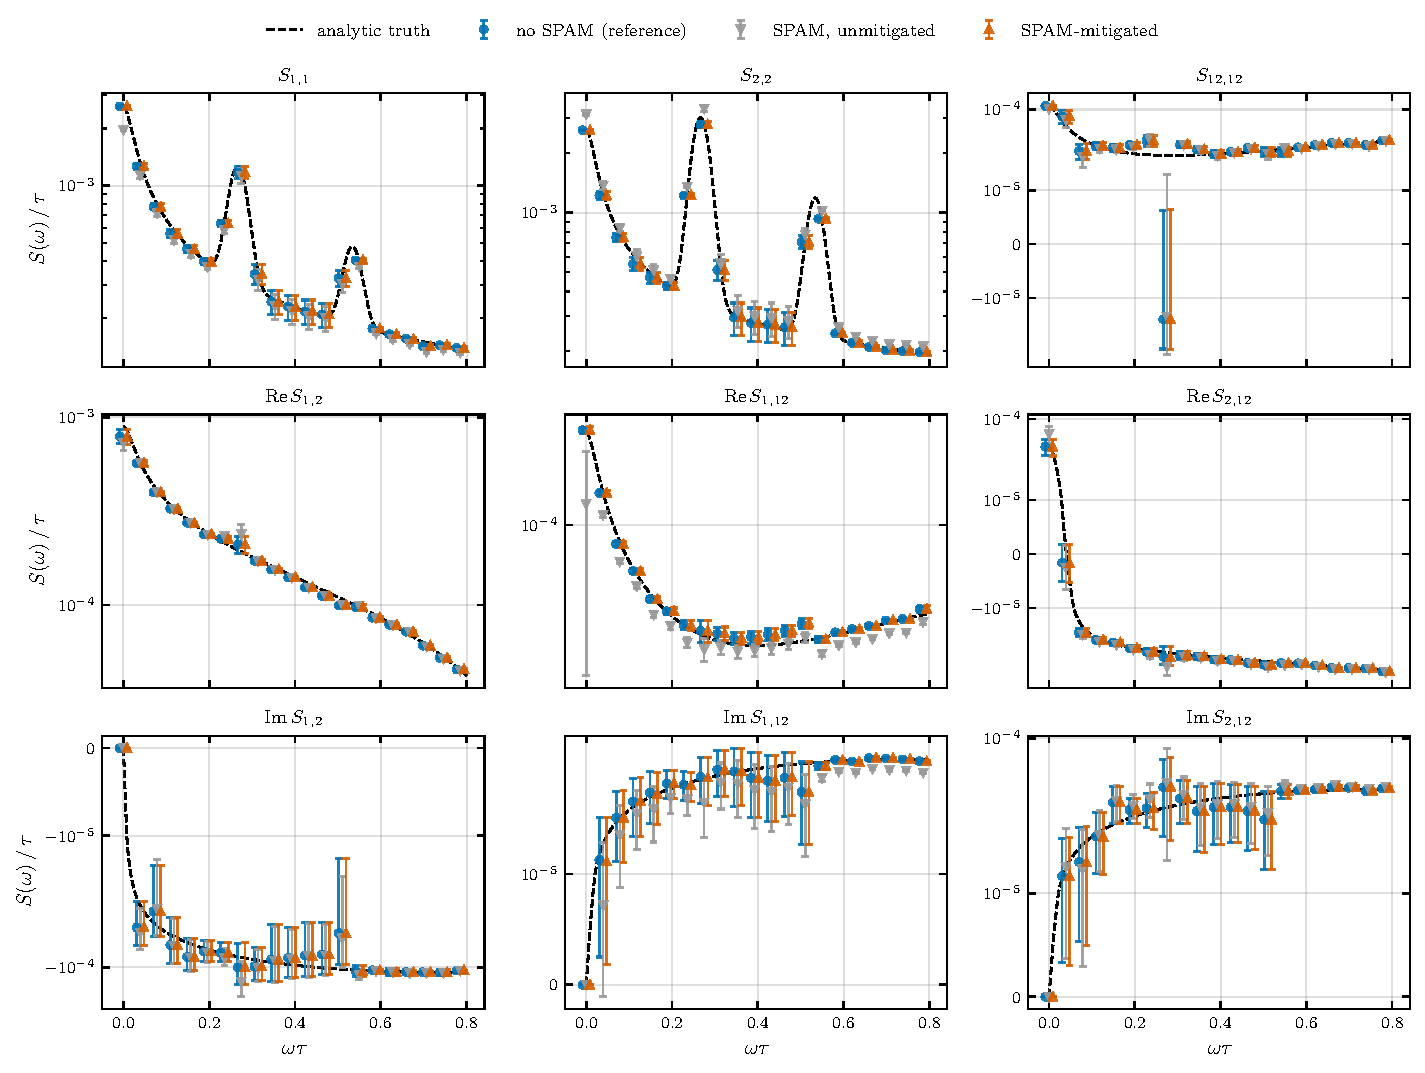
\includegraphics[width=0.96\linewidth]{figs/fig_spam_comparison.pdf}
\caption{The three reconstruction arms at 64k shots against analytic truth
(dashed): reference (no SPAM, blue circles), raw (SPAM, unmitigated, grey
triangles), and SPAM-mitigated (orange). Bars are the quoted total
(statistical $+$ systematic) uncertainties; arms are slightly offset in
$\omega$ for legibility. Top row: the three self-spectra; middle/bottom
rows: real and imaginary parts of the cross-spectra. The raw arm's bias is
largest at DC and the lowest harmonics (up to $34\sigma$); the mitigated arm
sits on the reference everywhere.}
\label{fig:spam}
\end{figure}

\section{What the gate design needs from the spectra, and what the
physics does}\label{sec:design}

With a trustworthy reconstruction in hand, the natural question is how much
of it the control design actually consumes. We answer it with two
experiments, run for both gates at fixed gate times (the entangling gate at
$\TG = 80\tau$ and $320\tau$; the idle gate at $\TG = 640\tau$ with $M=2$
repetitions and $2560\tau$ with $M=32$, the blind winners' repetition
numbers), with identical optimizer settings within each block
(Fig.~\ref{fig:design}).

\textbf{Spectral knowledge.} We re-ran the blind NT optimization while
progressively stripping spectral knowledge from the optimizer: all six
spectra $\to$ the SPAM-robust protocol's four $\to$ the three self-spectra
$\to$ the two single-qubit spectra alone. The benchmark (true infidelity of
the resulting gate, evaluated on the full model) barely moves. For the idle
gate at $640\tau$ the result is exact: the optimizer lands on the identical
winning sequence at the identical true infidelity under all four knowledge
sets; at $2560\tau$ the same pulse-count winner emerges within $1.5\%$ in
true infidelity. For the entangling gate, dropping the cross-spectra changes
nothing at either gate time, and even single-qubit-only knowledge costs just
$6\%$ at $80\tau$ (nothing at $320\tau$). The reason is structural: the
single-qubit spectra dominate the filter placement, and the CZ phase
constraint pins the $y_{12}$ filter's DC weight regardless of what the
optimizer believes about $S_{12,12}$.

\textbf{SPAM-biased spectra.} We then handed the optimizer the raw arm's
biased reconstruction. The result is the \emph{same gate} for both
operations: the identical NT(148,150) entangling winner at the identical
true infidelity ($4.27\times10^{-2}$ at $320\tau$), and the identical
NT(314,297)$^2$ idle winner at $5.18\times10^{-2}$ at $640\tau$, as the
respective reference-arm designs (Fig.~\ref{fig:design}, right column). The
SPAM bias is smooth, so it does not move the optimum. (These blocks draw
independent restarts, hence the slight offset from the curve numbers of
Sec.\,\ref{sec:gates}.)

The design is therefore forgiving, by construction: a blind protocol that
collapsed under partial knowledge or smooth bias would be useless in
practice. What full, unbiased characterization buys is everything around the
design:

\begin{itemize}[leftmargin=1.4em, itemsep=0.1em, topsep=0.2em]
\item \textbf{The error budget.} Undecoupled, the two-qubit channels
($S_{12,12}$ plus cross-spectra) carry a negligible $1.2\%$ of the gate
error at $\TG = 320\tau$. Under the best decoupling they carry
\textbf{20.4\%}: decoupling suppresses the single-qubit channels so
effectively that the two-qubit channels are promoted to a fifth of the
residual budget. Channel-resolved error budgeting of any decoupled gate
\emph{requires} two-qubit QNS.
\item \textbf{The prediction.} The reference arm predicts its entangling
gate's infidelity to $0.7\%$; the raw arm, designing the same gate,
mispredicts it by $1.9\%$. (For the idle gate the two arms happen to predict
equally well, within $\sim$3\%; but only the unbiased arm can
\emph{certify} its prediction, since with biased central values the quoted
uncertainties carry no meaning.) Every uncertainty band in
Sec.\,\ref{sec:gates} exists only because the bars in
Table~\ref{tab:recon} are unbiased with stated coverage.
\item \textbf{The spectroscopy itself.} At up to $34\sigma$, the raw arm's
spectra are not approximately right; they are confidently wrong.
\end{itemize}

Put together, the SPAM-robust four-spectrum protocol plus NT optimization is
a self-sufficient pipeline (it designs the same gate and predicts it from
immune data) when one accepts budget-level rather than channel-resolved
error accounting; SPAM-mitigated QNS recovers the full six-spectrum budget.

\begin{figure}[h!]
\centering
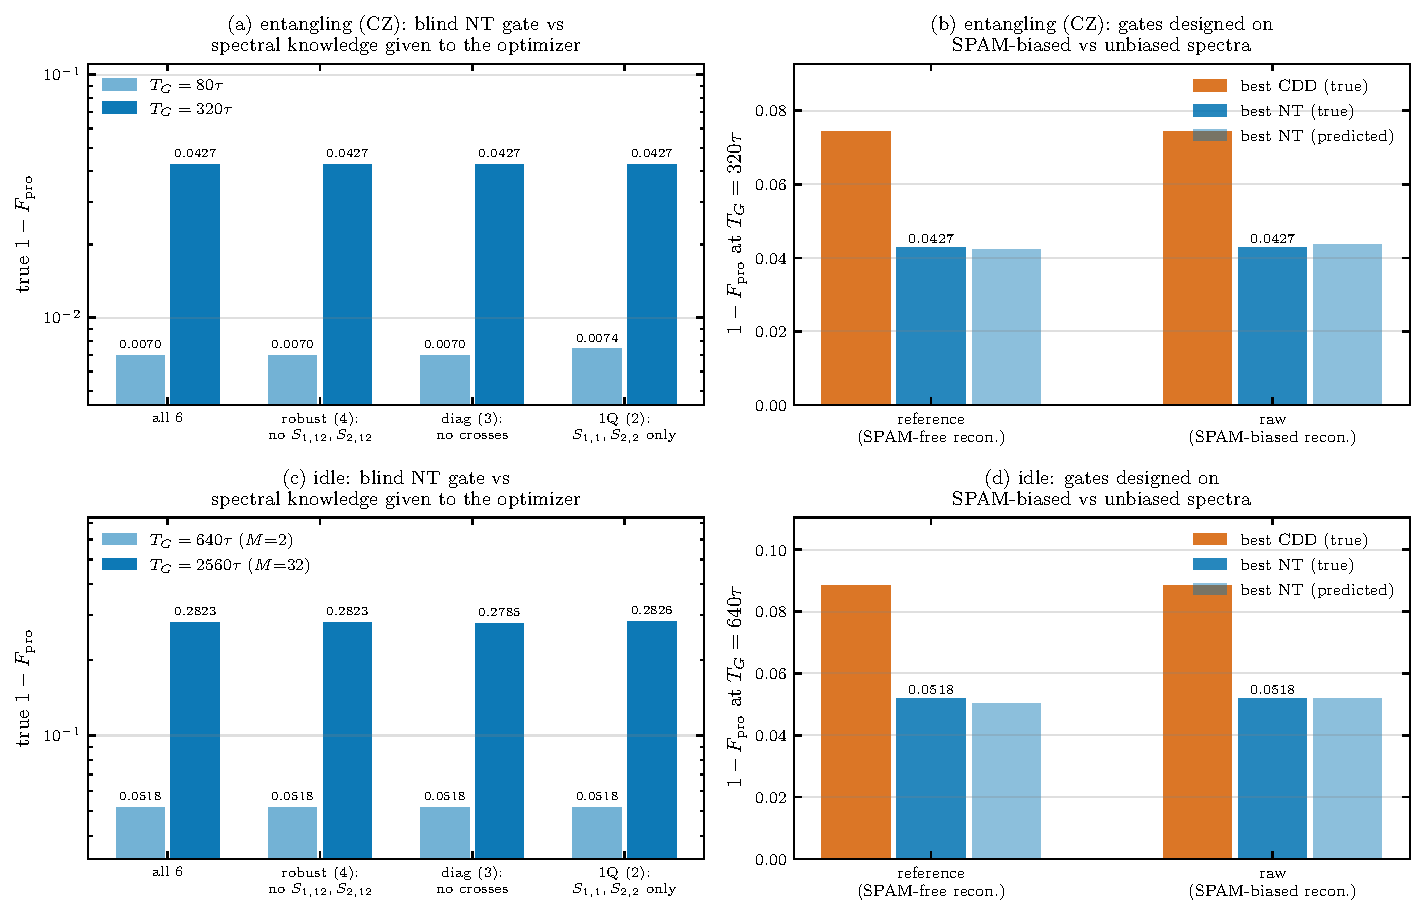
\includegraphics[width=0.92\linewidth]{figs/fig_design_experiments.pdf}
\caption{Both experiments for both gates: entangling (top row) and idle
(bottom row, at the blind winner's repetition number $M$). Left column: true
infidelity of the blind NT winner as the optimizer's spectral knowledge is
reduced (light/dark: the two gate times; log scale). The flatness across
knowledge sets is the result: the design is complete at the robust
protocol's four spectra for both gates, and nearly so with single-qubit
spectra alone (for the idle gate the winner is the same sequence under
every knowledge set: identical at $640\tau$, equal pulse counts within
$1.5\%$ at $2560\tau$). Right column: gates designed on the SPAM-biased
(raw) vs.\ SPAM-free (reference) reconstructions yield the same winner at
the same true infidelity for both gates; the bias surfaces only in the
predicted values (light bars).}
\label{fig:design}
\end{figure}

\section{The gates: margins for both operations}\label{sec:gates}

Figure~\ref{fig:gates} summarizes the regeneration. For both operations
(the entangling CZ gate and the idle gate, the latter optimized over the
repetition number $M$ at each gate time), the blind NT design beats the
best blind-selected CDD sequence at every operationally relevant gate time
and degrades gracefully to parity as $\TG$ crosses $T_2$.

\begin{figure}[h!]
\centering
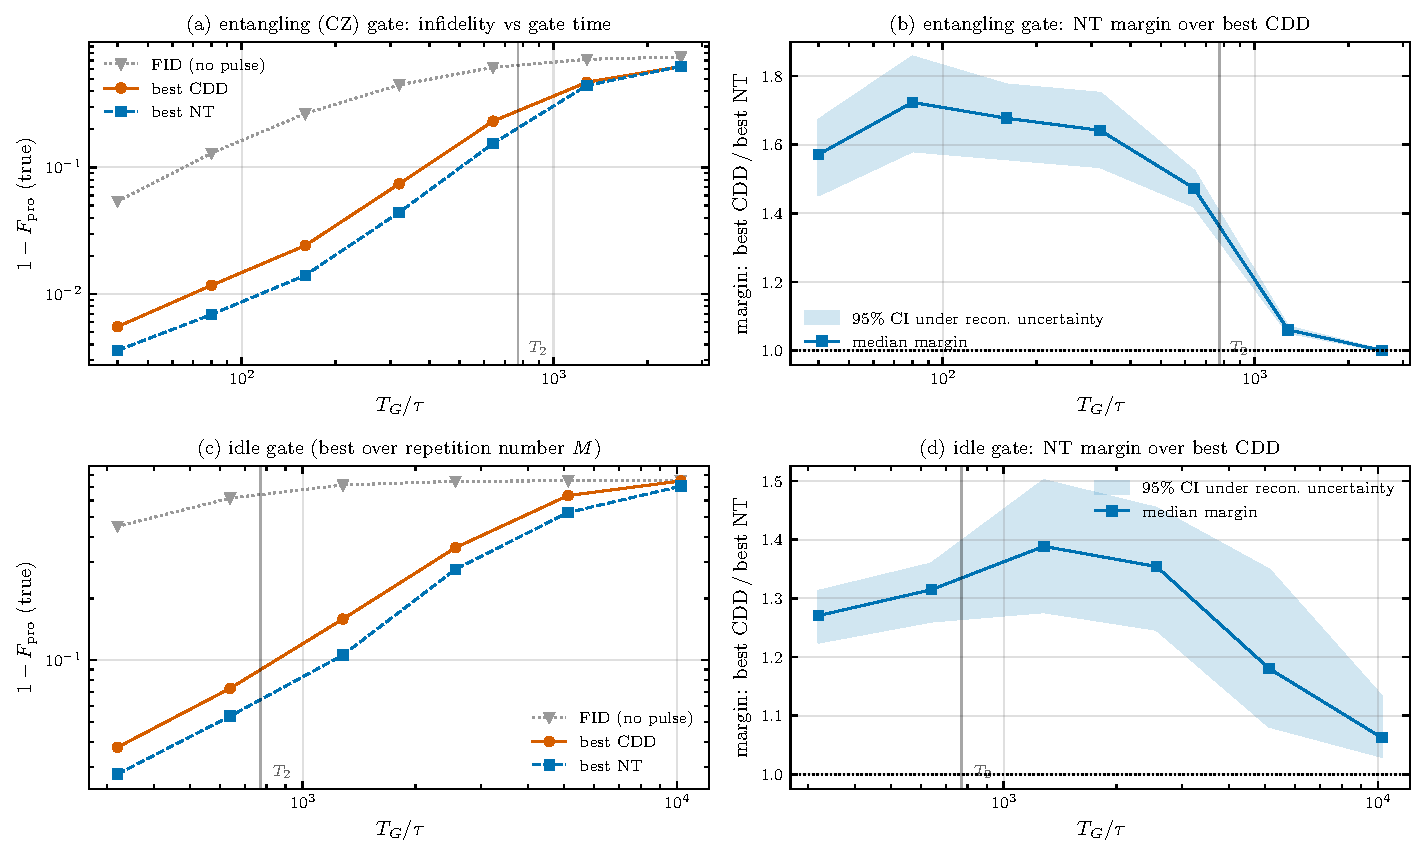
\includegraphics[width=\linewidth]{figs/fig_gates.pdf}
\caption{Noise-tailored gates on the anchored model, all design blind, all
scoring on truth. (a,c): true process infidelity vs.\ gate time for the
entangling and idle gates: free induction (grey), best CDD
(blind-selected, orange), best NT (blind-optimized, blue); the vertical line
marks $T_2 = 771\tau$. (b,d): the corresponding NT-over-CDD margin, with the
95\% confidence band obtained by propagating the reconstruction's quoted
statistical and systematic uncertainties (systematics drawn coherently per
channel, tail fits redone per draw) through both fixed winner sequences;
the band is on the \emph{ratio}, so common-spectrum fluctuations cancel.}
\label{fig:gates}
\end{figure}

The margins, with their 95\% confidence intervals under reconstruction
uncertainty:

\begin{itemize}[leftmargin=1.4em, itemsep=0.1em, topsep=0.2em]
\item \textbf{Entangling (CZ):} $1.54\times$ [1.45, 1.67] at $40\tau$;
$1.70\times$ [1.58, 1.86] at $80\tau$; $1.72\times$ [1.56, 1.77] at
$160\tau$; $1.68\times$ [1.54, 1.75] at $320\tau$; $1.50\times$ [1.42,
1.52] at $640\tau$; closing to $1.06\times$ [1.05, 1.07] at $1280\tau$. At
$2560\tau \approx 3.3\,T_2$ the blind optimizer's winner is the best CDD
sequence itself (exact parity).
\item \textbf{Idle:} $1.35\times$ [1.23, 1.31] at $320\tau$; $1.37\times$
[1.26, 1.36] at $640\tau$; $1.50\times$ [1.28, 1.50] at $1280\tau$;
$1.27\times$ [1.25, 1.45] at $2560\tau$; still $1.21\times$ [1.08, 1.35] at
$5120\tau$ and $1.06\times$ [1.03, 1.13] at $10240\tau = 13\,T_2$, deep in
the decoherence-dominated regime.
\end{itemize}

In each entry the central value is the \emph{true} margin and the bracket is
the 95\% interval of the \emph{predicted} margin under reconstruction
uncertainty; at 64k shots the two agree closely everywhere, with a mild
conservative tendency on the short idles (true margins at or just above
their predicted bands; the prediction errs on the safe side there).

\begin{table}[h!]
\centering\small
\begin{tabular}{lcccc}
\toprule
operation & FID & best CDD & best NT & margin \\
\midrule
idling $640\tau$ & $6.17\mathrm{e}{-1}$ & $7.29\mathrm{e}{-2}$ & $\mathbf{5.34\mathrm{e}{-2}}$ & $1.37\times$ \\
idling $2560\tau$ & $7.46\mathrm{e}{-1}$ & $3.54\mathrm{e}{-1}$ & $\mathbf{2.77\mathrm{e}{-1}}$ & $1.27\times$ \\
entangling $320\tau$ & $4.49\mathrm{e}{-1}$ & $7.42\mathrm{e}{-2}$ & $\mathbf{4.41\mathrm{e}{-2}}$ & $1.68\times$ \\
\bottomrule
\end{tabular}
\caption{Sweet-spot numbers on the anchored model (true process
infidelities, blind designs).}
\label{tab:regen}
\end{table}

The earlier draft's $10^2$--$10^3$ NT suppressions do not survive the move
to measured noise: they were artifacts of synthetic spectra carrying
negligible weight in the NT passband, and the anchored noise is far harsher
in absolute terms. The headline factor above is robust: the 95\% CI lower
edges stay at or above $1.42\times$ (CZ, $40$--$640\tau$) and $1.23\times$
(idle, $320$--$2560\tau$) across the operational windows. The structural
argument now carries the weight: decoupling promotes the two-qubit channels
to $20\%$ of the residual budget, and NT shapes the $y_{12}$ filter to
address exactly the channels decoupling cannot.

\vspace{0.3em}
The narrative the paper can now tell: spectra anchored feature-by-feature
to published measurements $\to$ a blind, SPAM-immune reconstruction
statistically consistent with truth $\to$ a design provably insensitive to
the spectra the robust protocol cannot see and the bias it cannot avoid
$\to$ noise-tailored idle and entangling gates beating the best decoupling
by $1.3$--$1.7\times$, with confidence bands inherited from the
reconstruction's stated uncertainties.

\vspace{0.4em}
\hrule
\vspace{0.3em}
{\footnotesize All optimization blind; true infidelities evaluated exactly on
the analytic model; all reconstructions at 64k shots per sequence.}

\end{document}
